\chapter{Projeto do sistema}\label{cap:projeto}

O sistema proposto será composto por dois módulos.
O primeiro corresponde à etapa de captura de fotos, detecção facial e upload das faces a serem processadas pelo segundo módulo, que, por sua vez, extrai características como idade, emoções e gênero e tenta verificar se a mesma face já foi analisada no passado.

\section{Módulo 1}\label{sec:modulo1}

O módulo 1 é o foco deste trabalho. Sua principal função é capturar as fotos a serem analisadas no segundo módulo.
Para minimizar o volume de dados trafegados pela rede e concentrar os esforços dos algoritmos de análise apenas nas áreas de interesse, o primeiro módulo não pode enviar todas as imagens capturadas, sendo necessário um pré-processamento que ignore as fotos que não contenham faces e também remova o fundo das fotos que contenham faces.

\subsection{Raspberry Pi}

Câmeras comuns não possuem poder computacional para realizar o pré-processamento desejado e computadores tradicionais são caros, grandes e muito pesados para esse propósito.

O meio termo ideal são os computadores de baixo custo em placa única, que podem ser posicionados de forma discreta e, apesar de limitados, são capazes de executar sistemas operacionais como o Linux ARM.

\begin{figure}[htbp]
    \centering
    \caption{Raspberry Pis com câmera}
    \label{fig:raspberry}
    \begin{subfigure}[t]{0.49\textwidth}
    \centering
    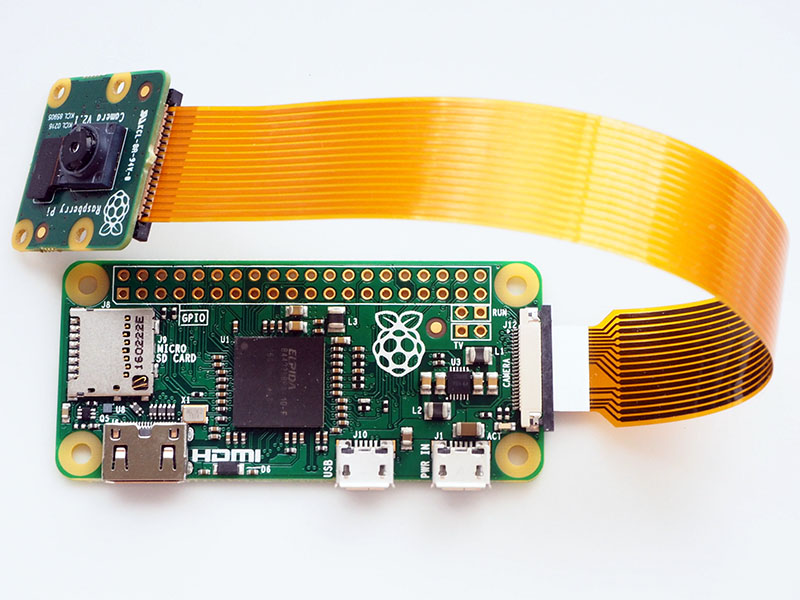
\includegraphics[width=0.95\linewidth]{imagens/raspberry_zero.jpg}
    \caption{Raspberry Pi Zero. Fonte: \cite{upton2016zero}} \label{fig:raspberry:a}
    \end{subfigure}
    \begin{subfigure}[t]{0.49\textwidth}
    \centering
    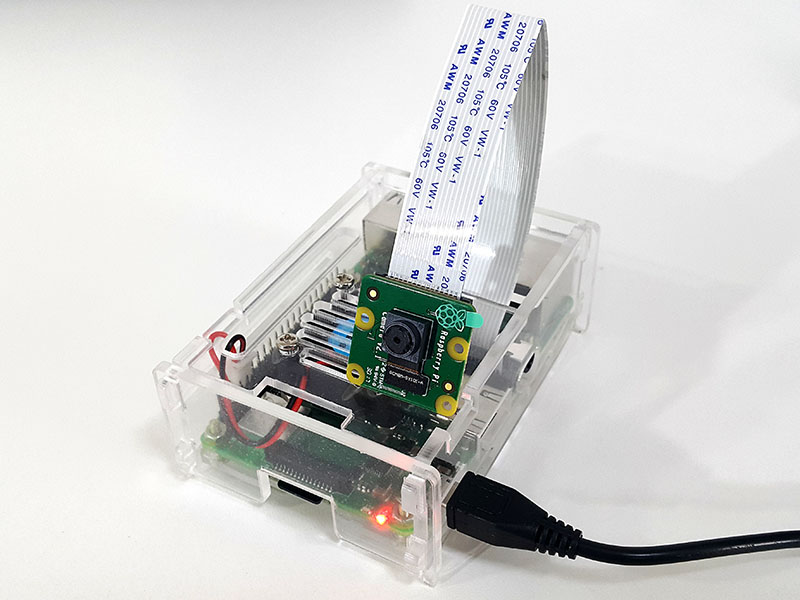
\includegraphics[width=0.95\linewidth]{imagens/raspberry.jpg}
    \caption{Raspberry Pi 3 modelo B+ em um case de acrílico} \label{fig:raspberry:b}
    \end{subfigure}
\end{figure}

O computador escolhido para este projeto foi o Raspberry Pi nos modelos Raspberry Pi Zero (\autoref{fig:raspberry:a}) e Raspberry Pi 3 B+ (\autoref{fig:raspberry:b}) devido ao seu baixo custo, alta disponibilidade e por possuir interface para câmera (CSI). O projeto completo custou menos de R\$ 500,00.

O Raspberry Pi Zero possui um processador ARM single-core de 1 GHz e 512 MB de memória SDRAM, enquanto que o Raspberry Pi 3 modelo B+ possui um processador quad-core 64-bit de 1,4 GHz e 1 GB de memória SDRAM.

O sistema operacional escolhido para ser instalado no Raspberry Pi foi o Raspbian Stretch Lite, uma distribuição de Linux baseada no Debian otimizada especificamente para o Raspberry Pi.

\subsection{Detecção facial}

O programa para selecionar apenas as regiões com faces deve utilizar um algoritmo eficiente de detecção facial capaz de ser executado a pelo menos um quadro por segundo no hardware e sistema operacional escolhidos.

O algoritmo de detecção facial selecionado para o primeiro módulo foi o Viola-Jones, pois, como estudado em capítulos anteriores, ele é eficiente o suficiente para ser executado em tempo real e está implementado na biblioteca multiplataforma OpenCV.

O \autoref{cod:detector_opencv_picamera} apresenta a implementação do sistema de detecção facial utilizando a câmera do Raspberry Pi.

\section{Módulo 2}\label{sec:modulo2}

O segundo módulo \ldots